
% PLoS Biology: http://journals.plos.org/plosbiology/s/submission-guidelines - No restrictions! Send definitely here first! IF:9.34
% Proceedings B:  ~5000 words (incl. everything!) IF:5.05
% Evolution (thesis format) IF:4.6

% texcount -incbib STD_draft.tex

% Points for the cover letter:
% -Mammalian evolution is back in trend again \citep{Wilson2013,O'Leary08022013,dosReis2014,Close2015,Lee2015R759}.
% -Effect of extinctions on species evolution (climate change blablablabla)
% -Our results are in opposition with the "myth" of the rise of the age of mammals due to dinosaurian oppresion
% -We propose a novel approach to look at disparity using phylogenetic structure and continuous sampling
%


\documentclass[12pt,letterpaper]{article}
\usepackage{natbib}

%Packages
\usepackage{pdflscape}
\usepackage{fixltx2e}
\usepackage{textcomp}
\usepackage{fullpage}
\usepackage{float}
\usepackage{latexsym}
\usepackage{url}
\usepackage{epsfig}
\usepackage{graphicx}
\usepackage{amssymb}
\usepackage{amsmath}
\usepackage{bm}
\usepackage{array}
\usepackage[version=3]{mhchem}
\usepackage{ifthen}
\usepackage{caption}
\usepackage{hyperref}
\usepackage{amsthm}
\usepackage{amstext}
\usepackage{enumerate}
\usepackage[osf]{mathpazo}
\usepackage{dcolumn}
\usepackage{lineno}
\usepackage{dcolumn}
\newcolumntype{d}[1]{D{.}{.}{#1}}

\pagenumbering{arabic}


%Pagination style and stuff
\linespread{2}
\raggedright
\setlength{\parindent}{0.5in}
\setcounter{secnumdepth}{0} 
\renewcommand{\section}[1]{%
\bigskip
\begin{center}
\begin{Large}
\normalfont\scshape #1
\medskip
\end{Large}
\end{center}}
\renewcommand{\subsection}[1]{%
\bigskip
\begin{center}
\begin{large}
\normalfont\itshape #1
\end{large}
\end{center}}
\renewcommand{\subsubsection}[1]{%
\vspace{2ex}
\noindent
\textit{#1.}---}
\renewcommand{\tableofcontents}{}
%\bibpunct{(}{)}{;}{a}{}{,}

%---------------------------------------------
%
%       START
%
%---------------------------------------------

\begin{document}

%Running head
\begin{flushright}
Version dated: \today
\end{flushright}
\bigskip
\noindent RH: Cretaceous-Palaeogene extinction does not affect mammalian disparity.

\bigskip
\medskip
\begin{center}


\noindent{\Large \bf Mammalian morphological diversity does not increase in response to the Cretaceous-Paleogene (K-Pg) extinction event and the extinction of the (non-avian) dinosaurs.} 
% TG: It's PalAEogene in the Oxford dictionary but PalEogene in the International Commission on Stratigraphy Chart.
% NC: OK, make a decision and stick to it.
% TG: shorter version:
% Mammalian morphological diversity does not change in response to the Cretaceous-Paleogene extinction event.
% NC: Yep that's grand too, I was just trying to get the word dinosaur in the title!
\bigskip

\noindent {\normalsize \sc Thomas Guillerme$^1$$^,$$^2$$^*$, and Natalie Cooper$^1$$^,$$^2$$^,$$^3$}\\
\noindent {\small \it 
$^1$School of Natural Sciences, Trinity College Dublin, Dublin 2, Ireland.\\
$^2$Trinity Centre for Biodiversity Research, Trinity College Dublin, Dublin 2, Ireland.\\
$^3$Department of Life Sciences, Natural History Museum, Cromwell Road, London, SW7 5BD, UK.}\\
\end{center}
\medskip
\noindent{*\bf Corresponding author.} \textit{guillert@tcd.ie}\\  
\vspace{1in}

%Line numbering
\modulolinenumbers[1]
\linenumbers

%---------------------------------------------
%
%       ABSTRACT
%
%---------------------------------------------

\newpage
\begin{abstract}
% NC: As ever I'm ignoring this until we are finished with the rest!
% TG: This is just here unedited for giving an idea of the length
% IGNORE THE ABSTRACT
Massive global extinctions have a turn-over effect on biodiversity. When some large group of taxa suffers from a high rate of extinction, it is expected that niches becomes available for potentially unrelated clades that can undergo an adaptive radiation to fill these vacant niches.
Therefore, in a context of current global biotic and abiotic changes, resolving this question is crucial to understand the effect of mass extinction events on biodiversity.
The causes and effects of such events are well understood for marine organisms with a good fossil record (e.g. Ammonoidea and Foraminifera) but the effects remains unclear on some iconic vertebrate groups.

Typically, placental mammals (eutherians) are shown by some studies to be undergoing an adaptive radiation after the Cretaceous-Palaeogene mass extinction event (K-Pg) by originating shortly before the K-Pg event and displaying high morphological evolutionary rates leading to high diversification during the Palaeogene. However, some other studies have demonstrated that eutherians originates during the Cretaceous and don't display significantly high diversification after the K-Pg event.

Here we propose a new approach to test if eutherians undergo an adaptive radiation after the K-Pg event. We use trees containing both living and fossil taxa based on all the available data (Total Evidence) and the state-of-the-art method in dating (tip dating) along side with a better proxy for niche occupancy (morphological diversity as opposed to taxonomic diversity) and finer grain analysis through time (introducing a time slicing method).

Our results shows that mammals don't display significantly changes in morphological disparity that expected under a Brownian motion after the K-Pg boundary. We therefore propose that eutherian mammals don't undergo an adaptive radiation during the Palaeogene.


%Our analyses provide a new approach to this debate by using both living and fossil species as well as morphological diversity (disparity) rather than taxonomic diversity as a proxy for mammalian diversity. 
%Our findings might change the long-lasting idea that the non-avian dinosaurs where restraining mammal evolution \citep{Lovergrove} or that their extinction liberate ecology niches for mammals to evolve in \citep{archibald2011extinction}.
% NC: This seems more like a conclusion/abstract than the discussion.

\end{abstract}

%IGNORE THE KEY WORDS
\noindent (Keywords: disparity, diversity, punctuated equilibrium, gradual evolution, time slicing)\\

\vspace{1.5in}

\newpage 

%---------------------------------------------
%
%       INTRODUCTION
%
%---------------------------------------------

\section{Introduction}
%
% TG: the number of citation is fairly high, should I cut it down to a minimum (no restrictions in PLoS Biology and Evolution though)
% NC: I reckon send it to PLoS Biology as is, then we can do what we did for Biology Letters. You have a lot of citations where you cite 4-5 papers so cutting those down will probably do it quite quickly. 
%
Throughout history, life on Earth has suffered a series of mass extinction events resulting in drastic declines in global biodiversity \citep[e.g.][]{RaupPT,BentonPT,rennetime2013,Brusatte2015}.
The long-term effects of mass extinctions, however, are more varied \citep{Erwin1998344}, and include species richness increases in some clades \citep{friedmanexplosive2010} and declines in others \citep{Benton85}, changes in morphological diversity \citep{Ciampaglio2001,Ciampaglio2004,kornextinction2013} and shifts in ecological dominance \citep[e.g.][]{Brusatte12092008,toljagictriassic-jurassic2013,bensonfaunal2014}.
These shifts are characterized by the decline of one clade that is replaced by a different unrelated clade with a similar ecological role (e.g. Brachiopoda and Bivalvia at the end Permian extinction; \citealt{Liow2015} %Sepkiski1981, CLAPHAM01102006
 but see \citealt{Payne22052014}). 
Shifts in ecological dominance are of particular interest because they are a fairly common pattern observed in the fossil record (e.g. Foraminifera; \citealt{Coxall01042006} %D'Hondt01011996
; Ichtyosauria; \citealt{thorneresetting2011}; Plesiosauria; \citealt{bensonfaunal2014}) and are often linked to major macroevolutionary processes such as adaptive \citep{Losos2010} or competitive \citep{Brusatte12092008} radiations.

One classical example of a shift in ecological dominance is at the Cretaceous-Palaeogene (K-Pg) mass extinction 66 million years ago \citep{rennetime2013}, where many terrestrial vertebrates (including the dominant non-avian dinosaur group; \citealt{archibald2011extinction,rennetime2013,Brusatte2015}) went extinct, allowing placental mammals to dominate the fauna \citep{archibald2011extinction,Lovergrove}. 
Some authors suggest this reflects placental mammals filling the ``empty'' niches left after the K-Pg extinction event \citep{archibald2011extinction,O'Leary08022013}, others suggest it reflects a release from predation and/or competition \citep{Slater2012MEE,Lovergrove}.
However, evidence for the diversification of placental mammals being driven by the K-Pg extinction event is mixed.
Thorough analysis of the fossil record \citep[e.g.][]{goswamia2011,O'Leary08022013} supports the idea that placental mammals diversified after the K-Pg extinction event as there are no undebated placental mammal fossils before it and many afterwards \citep{archibald2011extinction,goswamia2011,Slater2012MEE,O'Leary08022013,Wilson2013,Brusatte2015}. 
Conversely, evidence from molecular data suggests that the diversification of placental mammals started prior to the K-Pg extinction event without being drastically affected by it \citep[e.g.][]{Douady2003285,bininda2007delayed,meredithimpacts2011,Stadler12042011}.
Therefore, whether the diversification of placental mammals began before the K-Pg extinction event, or in response to the extinctions at K-Pg, is a matter of great debate \citep{dosReis2012,O'Leary08022013,Springer09082013,O’Leary09082013,dosReis2014}. 

There are two main reasons why there is still debate about the timing of the diversification of placental mammals. 
Firstly, palaeontological and neontological data show different patterns; palaeontological data generally suggest that placental mammals diversified after K-Pg \citep[e.g.][]{O'Leary08022013}, whereas neontological data suggest that K-Pg extinction event had little to no effect on mammalian diversification \citep{bininda2007delayed,meredithimpacts2011,Stadler12042011}.
We can solve this issue by using both palaeontological and neontological data in our analyses. 
The Total Evidence method allows us to use cladistic data for both living and fossil taxa, along with molecular data for living taxa, to build phylogenies \citep{ronquista2012}. %eernissetaxonomic1993
This method can also be combined with the tip-dating method \citep{ronquista2012,Wood01032013} to get more accurate estimates of diversification times for both fossil and living species \citep[but see][]{Arcila2015131}.
Here we use two recent Total Evidence tip-dated phylogenies of mammals \citep{Slater2012MEE,beckancient2014} to investigate palaeontological and neontological taxa simultaneously.

   % NC: Not really sure this fits anywhere?
    %Recently, two study have been published using the Total Evidence and tip-dating methods to study (1) variation in mammalian body mass \citep{Slater2012MEE} and (2) diversification rates \citep{beckancient2014} around the K-Pg boundary.
    % Slater: clear effect of the K-Pg boundary on body size constraint (body size evolution is OU before K-Pg and becomes BM afterwards)
    %\cite{Slater2012MEE} found good support for a shift in the mode of mammalian body mass evolution before and after the K-Pg boundary suggesting a clear effect of the K-Pg boundary on mammalian body mass diversification.
    % Beck: mixed (support for both no effect of K-Pg (ancient dates hypothesis) or for a possible more explosive model (accelerated rates))
    %Whereas, \cite{beckancient2014} found mixed result on diversification rates supporting both a diversification of placental mammals before (``ancient dates'' hypothesis) or after (``accelerated rates'' hypothesis) the K-Pg boundary. % TG: or maybe we don't give a flip about the hypothesis names (especially since they are the first words of the paper title)

A second issue is that diversity can be defined in many different ways.
In many studies it is measured as taxonomic diversity or species richness \citep{Stadler12042011,meredithimpacts2011,O'Leary08022013}, but often the more interesting aspect of diversity is related to the ecological niches the species occupy \citep{Wesley-Hunt2005,Brusatte12092008,toljagictriassic-jurassic2013}, particularly if we want to make hypotheses about macroevolutionary processes \citep{Pearman2008149,OlsonRadiation,Losos2010,glor2010phylogenetic,benton2015}.
Sometimes taxonomic diversity is used as a proxy for other kinds of diversity, however, species richness can be decoupled from morphological diversity \citep[e.g.][]{slaterCetacean,ruta2013,hopkinsdecoupling2013}, so it may not be the best proxy for ecological diversity.
We can instead use morphological diversity, also known as disparity \citep[e.g.][]{Wills1994,Erwin2007,Hughes20082013}, as a way to quantify changes in mammalian morphology that should relate to the ecology of the species.
However some methods for measuring disparity are outdated and make inappropriate assumptions.
Many methods for quantifying changes in morphological diversity were proposed $>$ 20 years ago \citep{Foote01071994,Wills1994} and are sometimes used without modifications \citep[e.g.,][]{brusatte50,Brusatte12092008,cisneros2010,thorneresetting2011,prentice2011,brusattedinosaur2012,toljagictriassic-jurassic2013,ruta2013,bentonmodels2014,bensonfaunal2014}. %, even when the statistical assumptions of the methods are violated (see Methods). TG: We don't talk about that anymore in the methods.
Additionally, previous methods are based on an underlying assumption that changes in disparity occur by punctuated evolution \citep[e.g.][]{Wesley-Hunt2005} which is not always the case \citep{Hunt21042015}.
Finally, most studies of disparity through time use unequal time units based on biostratigraphy \citep{Brusatte12092008,brusattedinosaur2012,toljagictriassic-jurassic2013}. 
This can be tautological as biostratigraphy is already based on changes in fossil assemblages and morphology through time.
To deal with these issues, we propose an updated approach to test whether mammals diversified in response to the K-Pg event, using morphological disparity, measured as cladistic disparity (see Methods), as our proxy for diversity.

Here we measure the disparity of living and fossil mammals before or after K-Pg, using data taken from two previously published studies \citep{Slater2012MEE,beckancient2014}. 
Using a novel time-slicing approach, we produce fine-grained estimates of disparity through time under two different models of morphological character evolution (either gradual or punctuated). 
We also test whether mammals display significant changes in disparity between the end of the Cretaceous and throughout the Cenozoic.
% TG: Added Wilson here. Not sure about the first part of the sentence. It might not be relevant here (but I thought it shows that mammalian Evolution in general is a hot topic).
% NC: It's a bit off topic and read like you're saying our study isn't novel so I cut it out. 
%Despite recent studies revealing unexpected mammalian diversification during the Jurassic \citep{Close2015,Lee2015R759}, 
Until now, this question has only been investigated using data from North American Therian mammals (excluding Monotremata) and without formally testing the effect of the K-Pg extinction event \citep{Wilson2013}.
To our knowledge, this study is the first to approach the debate about the effects of the K-Pg extinction event on mammalian evolution using Total Evidence phylogenies and by calculating disparity through time in a continuous way. %\citep[but see][for a similar question]{halliday2013testing}.
% NC: I'm unsure about this - it breaks up the sentence and is needlessly defensive. Maybe mention in the discussion instead? 
We find no significant changes in mammalian disparity between the end of the Cretaceous and any time during the Cenozoic. % NC: This needs updating. Also you're only looking at certain points in the Cenozoic now... 
These results suggest that the extinction of non-avian dinosaurs and other terrestrial vertebrate clades at the end of the Cretaceous did not affect mammalian morphological evolution.

%---------------------------------------------
%
%       METHODS
%
%---------------------------------------------

\section{Methods}

\subsection{Cladistic data and phylogenies}
We used the cladistic morphological matrices and the Total Evidence tip-dated trees \citep{ronquista2012} from \citet[][103 taxa with 446 morphological characters;]{Slater2012MEE} and \citet[][102 taxa with 421 morphological characters]{beckancient2014}.
We chose these two datasets because they have a similar number of taxa and morphological characters.
\cite{Slater2012MEE} ranges from 310 million years ago (Ma; Late Carboniferous) to the present and focuses on the clade Mammaliaformes at the family-level and is called hereafter the Mammaliaformes dataset.
\cite{beckancient2014} ranges from 170 Ma (Middle Jurassic) to the present and focuses on Eutheria at the genus-level and is called hereafter the Eutheria dataset.
We used the first and last occurrences reported in \cite{Slater2012MEE} and \cite{beckancient2014} as the temporal range of each taxon in our analysis.
Both phylogenies are illustrated in the supplementary material (see Fig S1 and S2 @@@).
Both trees contain few taxa compared to the overall species richness of living and fossil mammals \citep{bininda2007delayed,archibald2011extinction}.
This is because Total Evidence trees need a lot of data, particularly morphological data for living taxa that can be hard to locate \citep{GuillermeCooper}.
Therefore, most Total Evidence studies to date contain one or two orders of magnitude fewer taxa than phylogenies based solely on molecular data (e.g. thousands of taxa in \citealt{bininda2007delayed,meredithimpacts2011} \textit{vs.} hundreds in \citealt{ronquista2012,Slater2012MEE,Wood01032013,beckancient2014}).


\subsection{Estimating ancestral character states}
For both datasets we used the re-rooting method \citep{Yang01121995,Garland2000} to get Maximum Likelihood estimates of the ancestral states for each character at every node in the tree, using the \texttt{rerootingMethod} function from the \texttt{R} package \texttt{phytools} version 0.4-45 \citep{phytools,R}.
Where there was missing character data for a taxon we followed the method of \cite{Claddis} and treated missing data as any possible observed state for each character.
For example, if a character had two observed states ($0$ and $1$) across all taxa, we attributed the multi-state ``$0$\&$1$" value to the taxon with missing data, representing an equal probability of being either $0$ or $1$.
This allows the ancestral node of a taxon with missing data to be estimated with no assumptions other than that the taxon has one of the observed character states.
To prevent poor ancestral state reconstructions from biasing our results, especially when a lot of error is associated with the reconstruction, we only included ancestral state reconstructions with a scaled Likelihood $\geq$ $0.95$.
Ancestral state reconstructions with scaled Likelihoods below this threshold were replaced by missing data (``?'').

\subsection{Building the cladisto-space}
To explore variations in mammalian disparity through time (defined here as the variation in morphologies through time), we used a cladisto-space approach \citep[e.g.][]{Foote01071994,Foote29111996,Wesley-Hunt2005,Brusatte12092008,friedmanexplosive2010,toljagictriassic-jurassic2013,Hughes20082013}.
This approach is similar to constructing a morphospace based on continuous morphological data \citep[e.g.][]{friedmanexplosive2010}, except a cladisto-space is an approximation of the morphospace based on cladistic data (i.e. the discrete morphological characters used to build a phylogenetic tree).
Mathematically, a cladisto-space is an $n$ dimensional object that summarizes the cladistic distances between the taxa present in a cladistic matrix (see details below).
Although empirically inter-taxon distances are the same in a morphospace or a cladisto-space \citep{foth2012different,hetherington2015cladistic}, we prefer the term cladisto-space to make it clear that this space is estimated using cladistic data and not morphometric data and because both objects have slightly different properties.
For example, because of its inherent combinatory properties, a cladisto-space is a finite theoretical object limited by the product of the number of character states, whereas a morphospace is an infinite theoretical object.
Thus a cladisto-space will be overloaded if the number of taxa is higher than the product of the number of character states, although this is rarely an issue with empirical data (our cladisto-spaces have maximal capacities of $1.9$$\times$$10^{181}$ taxa for the Mammaliaformes dataset, i.e. 101 orders of magnitude more taxa than the number of particles in the universe; and $4.5$$\times$$10^{159}$ taxa for the Eutheria dataset).

To estimate the cladisto-spaces for each of our datasets we first constructed pairwise distance matrices of length $k$, where $k$ is the total number of tips and nodes in the datasets.
For each dataset separately, we calculated the $k$$\times$$k$ distances using the Gower distance \citep{Gower71}, i.e. the Euclidean distance between two taxa divided by the number of shared characters. 
This allows us to correct for distances between two taxa that share many characters and could be closer to each other than to taxa with fewer characters in common (i.e. because some pairs of taxa share more characters in common than others, they are more likely to be similar).
For cladistic matrices, using this corrected distance is preferable to the raw Euclidean distance because of its ability to deal with discrete or/and ordinated characters as well as with missing data \citep{anderson2012using}.
However, the Gower distance cannot calculate distances when taxa have no overlapping data.
Therefore, we used the \texttt{TrimMorphDistMatrix} function from the \texttt{Claddis} R package \citep{Claddis} to remove pairs of taxa with no cladistic characters in common.
This led to us removing 11 taxa from the Mammaliaformes dataset but none from the Eutheria dataset.

%\subsubsection{Ordination}
After calculating our distance matrices we transformed them using classical multidimensional scaling \citep[MDS;][]{torgerson1965multidimensional,GOWER01121966,cailliez1983analytical}.
This method (also referred to as PCO; e.g. \citealt{Brusatte2015}; or PCoA; e.g. \citealt{paradisape:2004}) is an eigen decomposition of the distance matrix.
Because we used Gower distances instead of raw Euclidean distances, negative eigenvalues can be calculated.
To avoid this problem, we first transformed the distance matrices by applying the Cailliez correction \citep{cailliez1983analytical} which adds a constant $c^*$ to the values in a distance matrix (apart from the diagonal) so that all the Gower distances become Euclidean ($d_{Gower}+c^*=d_{Euclidean}$; \citealt{cailliez1983analytical}). 
We were then able to extract $n$ eigenvectors for each matrix (representing the $n$ dimensions of the cladisto-space) where $n$ is equal to $k-2$, i.e. the number of taxa in the matrix ($k$) minus the last two eigenvectors that are always null after applying the Cailliez correction.
Contrary to previous studies \citep[e.g][]{brusatte50,cisneros2010,prentice2011,anderson2012using,Hughes20082013,bentonmodels2014}, we use all $n$ dimensions of our cladisto-spaces and not a subsample representing the majority of the variance in the distance matrix (e.g. selecting only $m$ dimensions that represent up to 90\% of the variance in the distance matrix; \citealt{Brusatte12092008,toljagictriassic-jurassic2013}).

Note that our cladisto-spaces represent an ordination of all possible mammalian morphologies coded in each study through time.
It is unlikely that all morphologies will co-occur at each time point, therefore, the disparity of the whole cladisto-space is expected to be greater than the disparity at any specific point in time.

\subsection{Calculating disparity}
Disparity can be estimated in many different ways \citep[e.g.][]{Wills1994,Ciampaglio2004,thorneresetting2011,hopkinsdecoupling2013,huang2015origins}, however most studies estimate disparity using four metrics: the sum and products of ranges and variances, each of which gives a slightly different estimate of how the data fits within the cladisto-space \citep{Foote01071994,Wills1994,brusatte50,Brusatte12092008,cisneros2010,thorneresetting2011,prentice2011,brusattedinosaur2012,toljagictriassic-jurassic2013,ruta2013,bentonmodels2014,bensonfaunal2014}.
% KEEP THE RANT BELOW
%The sum and products of ranges and variances are based on the ranges and variances of the eigenvectors calculated from a distance matrix. 
%However, these metrics do not take into account the covariance among eigenvectors. % TG: I think I need a bit of chat with Dr Jackson here. He's statement that sum of variance is not correct because it ignores covariance might be actually not a good argument. He's still right but in practice, the covariance between the eigenvectors seems to be always 0 (because each axis are orthogonal to each other). It doesn't change anything for our story but it might be good to no state that these variance calculations are wrong if they are ok (in practice, again, in theory, they remain wrong). % NC: Up to you. You could cut this whole section and just say we use centroids like Wills to estimate disparity.
%This is only statistically valid if the eigenvectors are independent.
%In multidimensional scaling, all $n$ eigenvectors are calculated from the same distance matrix and are therefore not independent, thus covariances among eigenvectors should be included when estimating disparity.
%
Nonetheless, these methods suffer several methodological caveats.
First, the range metrics are affected by the uneven sampling of the fossil record \citep{Butler2012}
Second, because we include all $n$ dimensions in the analysis (see above), the products of ranges and variances will tend towards zero since the scores of the last dimension are usually really close to zero themselves. 
These features make using the sum and products of ranges and variances unfeasible in our study.
Instead, we use a different metric that comes with no statistical assumptions for measuring the dispersion of the data in the cladisto-space: the median distance between tips and nodes and the centroid (similar but not equivalent to \citealt{Wills1994,kornextinction2013,huang2015origins}) calculated as:

\begin{equation}
   Disparity=median{\displaystyle\sqrt{\sum{(\mathbf{v}_{n}-Centroid_{n})^2}}}
    \label{disparity}
\end{equation}
where:
\begin{equation}
    Centroid_{n}=\frac{\displaystyle\sum(\mathbf{v}_{n})}{k} 
    \label{centroid}
\end{equation}

\noindent
and $\mathbf{v}_{n}$ is any of the $n$ eigenvectors (i.e. any of the $n$ dimensions of the cladisto-space), $Centroid_{n}$ is the mean value of the $n^{th}$ eigenvector (equation \ref{centroid}) and $k$ is the total number of tips and nodes.
Note that we also calculated the sum and products of ranges and variances and refer to these results in the supplementary material (@@@). % link to supp.

\subsection{Estimating disparity through time} 
Changes in disparity through time are generally investigated by calculating the disparity of taxa that occupy the cladisto-space during specific time intervals \citep[e.g][]{cisneros2010,prentice2011,Hughes20082013,hopkinsdecoupling2013,bentonmodels2014,bensonfaunal2014}.
These time intervals are usually defined based on biostratigraphy \citep[e.g.][]{cisneros2010,prentice2011,Hughes20082013,bentonmodels2014} but can also be arbitrarily chosen time periods of equal duration \citep{Butler2012,hopkinsdecoupling2013,bensonfaunal2014}.
However, this approach suffers from two main biases. 
First, if biostratigraphy is used to determine the time intervals, disparity may be distorted towards higher differences between time intervals because biostratigraphical periods are geologically defined based on differences in the morphology of fossils found in the different strata.
Second, this approach assumes that all characters evolve following a punctuated equilibrium model, because disparity is only estimated once for each interval resulting in all changes in disparity occurring between intervals, rather than also allowing for gradual changes within intervals \citep{Hunt21042015}.

To address these issues, we used a ``time-slicing'' approach that considers subsets of taxa in the cladisto-space at specific equidistant points in time, as opposed to considering subsets of taxa between two points in time.
This results in even-sampling of the cladisto-space across time and permits us to define the underlying model of character evolution (punctuated or gradual).  
In practice, time-slicing considers the disparity of any element present in the phylogeny (branches, nodes and tips) at any point in time.
When the phylogenetic elements are nodes or tips, the eigenvector scores for the nodes (estimated using ancestral state reconstruction as described above) or tips are directly used for estimating disparity.
When the phylogenetic elements are branches we chose the eigenvector score for the branch using one of two evolutionary models:
\begin{enumerate}
    \item{\textbf{Punctuated evolution.}} 
    This model selects the eigenvector score from either the ancestral node or the descendant node/tip of the branch regardless of the position of the slice along the branch. 
    Similarly to the time interval approach, this reflects a model of punctuated evolution where changes in disparity occur either at the start or at the end of a branch over a relatively short time period and clades undergo long periods of stasis during their evolution \citep{Gould1977,Hunt20112007}.
    We applied this model in three ways: 
    \begin{enumerate}[(i)]
      \item selecting the eigenvector score of the ancestral node of the branch (ACCTRAN).
      \item selecting the eigenvector score of the descendant node/tip of the branch (DELTRAN).
      \item randomly selecting either the eigenvector score of the ancestral node or the descendant node/tip of the branch (random).
    \end{enumerate}
    Method (i) assumes that changes always occur early on the branch (accelerated transition, ACCTRAN) and (ii) assumes that changes always occur later (delayed transition, DELTRAN).
    We prefer not to make either assumption so we report the results from (iii), although the ACCTRAN and DELTRAN results are available in the Supplementary Information @@@. % link
    \item{\textbf{Gradual evolution.}}
    This model also selects the eigenvector score from either the ancestral node or the descendant node/tip of the branch, but the choice depends on the distance between the sampling time point and the end of the branch.
    If the sampling time point falls in the first half of the branch length the eigenvector score is taken from the ancestral node, conversely, if the sampling time point falls in the second half of the branch length the eigenvector score is taken from the descendant node/tip.
    This reflects a model of gradual evolution where changes in disparity are gradual and cumulative along the branch.
    Under this model, the gradual changes could be either directional or random, however, directional evolution have been empirically shown to be rare \citep[only 5\% of the time][]{Hunt20112007}.
    We therefore considered that changes from a character state A to B were only dependent on the branch length.
\end{enumerate}
%What did we do (the main figure)
We applied our time-slicing approach separately to the two cladisto-spaces calculated for the Mammaliaformes and Eutheria datasets, time-slicing the phylogeny every five million years from 170 Ma to the present resulting in 35 subsamples of the cladisto-space.
For each subsample, we estimated its disparity assuming punctuated (ACCTRAN, DELTRAN and random) and gradual evolution as described above.
To reduce the influence of outliers on our disparity estimates, we bootstrapped each disparity measurement by randomly resampling with replacement a new subsample of taxa from the observed taxa in the subsample 1000 times.
We then calculated the median disparity value for each subsample along with the 50\% and 95\% confidence intervals.
We also recorded the number of phylogenetic elements (nodes and tips) in each subsample as a proxy for taxonomic diversity.
To compare our results to previous studies we also repeated our analyses using the time interval approach based on biostratigraphy \citep[e.g.][]{cisneros2010,prentice2011,Hughes20082013,bentonmodels2014} using each geological stage from the Middle Jurassic to the present.
We report the results of these analyses in the Supplementary Materials (@@@). % link

%Testing the difference section
\subsection{Testing the effects of the K-Pg extinction on mammalian disparity}
If the K-Pg extinction event had a significant effect on mammalian disparity, we should see a significant difference between disparity at the end of the Cretaceous and disparity at the start of the Paleogene.
To test this, we performed t-tests to look for differences in disparity among the time subsamples before and after the K-Pg boundary at 66 Ma, i.e. the subsamples at 70 and 65 Ma \citep[e.g. as used in][]{anderson2012using,zelditch2012geometric,smith2014joined}, for both the Mammaliaformes and Eutheria datasets and using both the gradual and punctuated evolutionary models.
Because the effect of a mass extinction event on a group's evolution might not be detectable directly after the event due to delays in recovery \citep[e.g.][estimated that ecosystems only fully recovered 8-9 Ma after the Permo-Triassic mass extinction]{chen2012timing}, we also tested whether there was a significant difference in disparity between the end of the Cretaceous and all subsamples from the Paleocene and the Eocene up to the Late Priabonian, 35 Ma.
% NC: Explain why you stop at 35 Ma and not 50 Ma (60 - 9 = 51 not 35). Stuff about wanting to include the PETM.
Because these analyses involved multiple comparisons, we used Bonferonni corrections \citep{holm1979simple} to ensure our significant results were robust to Type I error rate inflation. 


%Moved that from above for explaining the rarefaction
Finally, disparity may be higher in subsamples with more phylogenetic elements simply because there are more taxa represented.
To test whether this influenced our results, we repeated the t-tests using the rarefied Mammaliaformes and Eutheria disparities.
In the Mammaliaformes, the minimum number of taxa in each subsample from 170 Ma to present was eight.
In the Eutheria, the minimum number of taxa in each subsample was three, however, from 150 Ma until the present, the minimum number of taxa is eight.
To make both datasets comparable, we used eight as a minimum number of taxa for the rarefied bootstrap measurements, therefore in the Eutheria we ignored the subsample between 170 and 150 Ma that only contains three taxa.

% we first tested whether there was a significant effect of time on disparity using \cite{permanova}'s Permutational Analysis of Variance \citep[also referred to as PERMANOVA or NPANOVA; e.g.][]{brusatte50,ruta2013}.
% We calculated the Euclidean distance of the ordinated data with 1000 permutations on both datasets and on both evolutionary scenarios using the \texttt{adonis} function from the R package \texttt{vegan} \citep{vegan}.
% NC: I feel like there are details missing here - what's the explanatory variable and the response etc. 

% When we found a significant effect of time on disparity % NC: Again there's a bit missing here but should be easy to fix.
% , we ran a series of \textit{post-hoc} t-tests among the time subsamples before and after the K-Pg boundary \citep{anderson2012using,zelditch2012geometric,smith2014joined} as follows.
% We measured the difference between the last subsample of the Cretaceous (65 Ma) to all the slices of the Cenozoic to test whether there was either:
% \begin{enumerate}
%     \item{no effect of the K-Pg event: no significant difference between the last Cretaceous subsample and any of the Cenozoic subsamples.}
%     \item{a direct effect of the K-Pg event: significant difference between the last Cretaceous subsample and the first Cenozoic subsample.}
%     \item{a lag effect of the K-Pg event: a significant difference between the last Cretaceous subsample and some subsamples during the Cenozoic.}
% \end{enumerate}
% Because these \textit{post-hoc} t-tests involve multiple comparisons, we corrected each p-value by multiplying them by the number of comparisons \citep[Holm-Bonferonni correction;][]{holm1979simple}.

%---------------------------------------------
%
%       RESULTS
%
%---------------------------------------------

\section{Results}
%§1 - How does disparity change through time? % NC: Don't add epoch names for the sake of it - they're weird and not helpful in most cases.
Disparity in the Mammaliaformes reaches a plateau during the Middle Triassic around 240 Ma, and fluctuates slightly around its maximum during the rest of the Mesozoic and the Cenozoic (Fig \ref{fig:Fig_Raw_results} and Fig @@@ supplementary).
The number of tips and nodes in each time subsample (a proxy for taxonomic richness), however, show a more idiosyncratic pattern with a steady increase until the Middle Jurassic around 170 Ma, Fig @@@ supplementary) followed by random fluctuations during the rest of the Mesozoic and the Cenozoic (Fig \ref{fig:Fig_Raw_results}).
Disparity in the Eutheria reaches a plateau at the end of the Jurassic around 150 Ma, whereas the number of tips and nodes increases up to the K-Pg boundary and then decreases throughout the Cenozoic (Fig \ref{fig:Fig_Raw_results}).
For both Mammaliaformes and Eutheria the same patterns in changes in disparity appear in the rarefied analyses (Fig \ref{fig:Fig_Raw_results} and @@rar@@sup).
In both datasets the two evolutionary models (gradual or punctuated) also yield similar results (Fig \ref{fig:Fig_Raw_results}).

We found no significant differences in disparity between the last subsample of the Cretaceous (70 Ma) and the first subsample of the Paleogene (65 Ma; Tables \ref{tab:Tab_slater} and \ref{tab:Tab_beck}), using both datasets and under both evolutionary models. 
% This suggests that there is no direct effect of the K-Pg extinction event on mammalian disparity.
% NC: I added some interpretation but really it belongs in the disccusion so i commented it out.
We also found no significant differences in disparity between the last subsample of the Cretaceous (70 Ma) and any subsamples of the Paleocene and Eocene in Mammaliaformes under both evolutionary models and in Eutheria under a gradual evolutionary model (Tables \ref{tab:Tab_slater} and \ref{tab:Tab_beck}).
%This suggests that in these analyses, there was also no delayed effect of the K-Pg extinction event on mammalian disparity.
However, in Eutheria under the punctuated evolutionary model, we found a small significant difference (after applying Bonferonni corrections) in disparity between the last subsample of the Cretaceous (70 Ma) and the subsamples at 50 Ma and 40 Ma (an increase in disparity of 0.16 and 0.20 respectively; Table \ref{tab:Tab_beck}). % NC: Do these numbers have units?
However, this result is not significant in the rarefied analyses (Tables supplementary@@@). 
Otherwise the results of the rarefied analyses are the same as when using the complete datasets. 

% NC: In the discussion be specific, how many nodes and tips are we talking about here? Is it because there are lots of nodes in these two bins and not others, or because there are few? Is it because there is one huge species missing? Look at the data.

\begin{figure}[!htbp]
\centering
    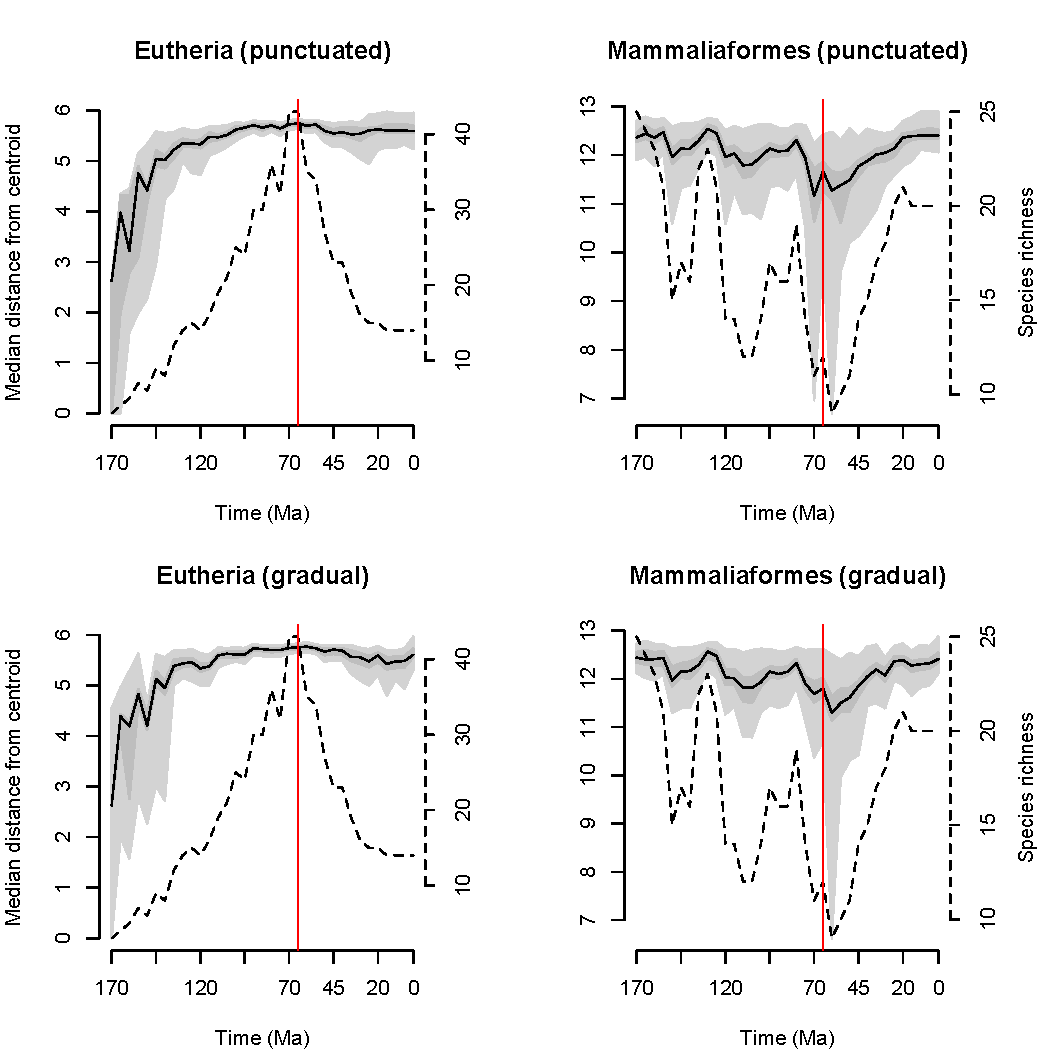
\includegraphics[keepaspectratio=true]{Figures/Main_results.pdf}
\caption{\tiny{Disparity through time in Eutheria and Mammaliaformes calculated using a model of punctuated (upper panels) or gradual  (lower panels) evolution. The x axis represents time in millions of years before the present (Ma). The y axis represents disparity, measured as the median distance between the centroid of the ordinated space and the tips/nodes in each time subsample. The solid black lines show the mean disparity estimated from 1000 bootstrapped pseudoreplicates and confidence intervals (CI) are represented by the grey polygons (50\% CI in dark grey and 95\% CI in light grey). The dashed line and the right hand axis represents the number of tips/nodes in each time slice. The red vertical line indicates the Cretaceous-Paleogene (K-Pg) boundary (66 Ma). Note that scale bars differ among panels.}}
\label{fig:Fig_Raw_results}
\end{figure}
% NC: Figure legend has slipped off the bottom of the page so I've made the text tiny for now!

\begin{table}[ht]
\caption{Results of t-tests comparing disparity at the last subsample of the Cretaceous (70 Ma) to subsamples of the Paleocene and Eocene, under both gradual and punctuated evolutionary models, in Mammaliaformes. Difference = mean difference in disparity between the two subsamples being compared; df = degrees of freedom; p value = original p value prior to Bonferonni correction. }
\label{tab:Tab_slater}
\centering
\begin{tabular}{r|cccc|cccc}
  \hline
  Subsamples & \multicolumn{4}{c|}{Gradual evolution model} & \multicolumn{4}{c}{Punctuated evolution model} \\
  compared & difference & df & t & p value & difference & df & t & p value \\ 
  \hline
  70 \textit{vs.} 65 Ma & -0.420 & 21 & -0.772 & 0.449 & -0.310 & 21 & -0.732 & 0.472 \\ 
  70 \textit{vs.} 60 Ma & 0.030 & 18 & 0.054 & 0.957 & 0.390 & 18 & 0.633 & 0.535 \\ 
  70 \textit{vs.} 55 Ma & 0.010 & 19 & 0.018 & 0.986 & 0.210 & 19 & 0.383 & 0.706 \\ 
  70 \textit{vs.} 50 Ma & -0.290 & 20 & -0.533 & 0.600 & -0.190 & 20 & -0.431 & 0.671 \\ 
  70 \textit{vs.} 45 Ma & -0.470 & 23 & -0.976 & 0.339 & -0.340 & 23 & -0.812 & 0.425 \\ 
  70 \textit{vs.} 40 Ma & -0.640 & 24 & -1.450 & 0.160 & -0.460 & 24 & -1.283 & 0.212 \\ 
  70 \textit{vs.} 35 Ma & -0.750 & 26 & -1.820 & 0.080 & -0.460 & 26 & -1.270 & 0.215 \\ 
   \hline
\end{tabular}
\end{table}

\begin{table}[ht]
\caption{Results of t-tests comparing disparity at the last subsample of the Cretaceous (70 Ma) to subsamples of the Paleocene and Eocene, under both gradual and punctuated evolutionary models, in Eutheria. Difference = mean difference in disparity between the two subsamples being compared; df = degrees of freedom; p value = original p value prior to Bonferonni correction. Significant differences (after applying Bonferonni corrections for multiple comparisons) are highlighted in bold.}
\label{tab:Tab_beck}
\centering
\begin{tabular}{r|cccc|cccc}
  \hline
  Subsamples & \multicolumn{4}{c|}{Gradual evolution model} & \multicolumn{4}{c}{Punctuated evolution model} \\
  compared & difference & df & t & p value & difference & df & t & p value \\ 
  \hline
  70 \textit{vs.} 65 Ma & -0.020 & 84 & -0.546 & 0.586 & 0.030 & 84 & 0.756 & 0.452 \\ 
  70 \textit{vs.} 60 Ma &  0.030 & 76 & 0.608 & 0.545 & 0.060 & 76 & 1.189 & 0.238 \\ 
  70 \textit{vs.} 55 Ma &  0.030 & 75 & 0.562 & 0.576 & 0.020 & 75 & 0.383 & 0.703 \\ 
  70 \textit{vs.} 50 Ma &  0.130 & 68 & 2.090 & 0.040$^1$ & 0.160 & 68 & 2.984 & \textbf{0.004}$^2$ \\ 
  70 \textit{vs.} 45 Ma &  0.180 & 64 & 2.719 & 0.008$^1$ & 0.160 & 64 & 2.641 & 0.010$^1$ \\ 
  70 \textit{vs.} 40 Ma &  0.150 & 64 & 2.280 & 0.026$^1$ & 0.200 & 64 & 3.172 & \textbf{0.002}$^3$ \\ 
  70 \textit{vs.} 35 Ma &  0.200 & 60 & 2.532 & 0.014$^1$ & 0.170 & 60 & 2.598 & 0.012$^1$ \\ 
   \hline
\end{tabular} \\
   $^1$p values non-significant after applying Bonferonni correction;
   $^2$p value is \textbf{0.018} after applying Bonferonni correction;
   $^3$p value is \textbf{0.032} after applying Bonferonni correction.
\end{table}


\begin{table}[ht]
\caption{Results of t-tests comparing disparity at the last subsample of the Cretaceous (70 Ma) to subsamples of the Paleocene and Eocene, under both gradual and punctuated evolutionary models, in Mammaliaformes. Difference = mean difference in disparity between the two subsamples being compared; df = degrees of freedom; p value = original p value prior to Bonferonni correction. }
\label{tab:Tab_slater}
\centering
\begin{tabular}{r|cccc|cccc}
  \hline
  Subsamples & \multicolumn{4}{c|}{Gradual evolution model} & \multicolumn{4}{c}{Punctuated evolution model} \\
  compared & difference & df & t & p value & difference & df & t & p value \\ 
  \hline
  70 \textit{vs.} 65 Ma & -0.420 & 21 & -0.772 & 0.449 & -0.310 & 21 & -0.732 & 0.472 \\ 
  70 \textit{vs.} 60 Ma & 0.030 & 18 & 0.054 & 0.957 & 0.390 & 18 & 0.633 & 0.535 \\ 
  70 \textit{vs.} 55 Ma & 0.010 & 19 & 0.018 & 0.986 & 0.210 & 19 & 0.383 & 0.706 \\ 
  70 \textit{vs.} 50 Ma & -0.290 & 20 & -0.533 & 0.600 & -0.190 & 20 & -0.431 & 0.671 \\ 
  70 \textit{vs.} 45 Ma & -0.470 & 23 & -0.976 & 0.339 & -0.340 & 23 & -0.812 & 0.425 \\ 
  70 \textit{vs.} 40 Ma & -0.640 & 24 & -1.450 & 0.160 & -0.460 & 24 & -1.283 & 0.212 \\ 
  70 \textit{vs.} 35 Ma & -0.750 & 26 & -1.820 & 0.080 & -0.460 & 26 & -1.270 & 0.215 \\ 
   \hline
\end{tabular}
\end{table}

% NC: What about this? Rule of thumb is that if the legends are the same and column headings are the same they should be the same table unless they're way too big to fit. These will be fine for the thesis if you get rid of double spacing. You may also want to highlight entire rows in grey shading if they are important - for the thesis not the paper.

% NC: Make column headings bold

\begin{table}[ht]
\caption{\tiny{Results of t-tests comparing disparity at the last subsample of the Cretaceous (70 Ma) to subsamples of the Paleocene and Eocene, under both gradual and punctuated evolutionary models, in Mammaliaformes and Eutheria. Difference = mean difference in disparity between the two subsamples being compared; df = degrees of freedom; p value = original p value prior to Bonferonni correction. Significant differences (after applying Bonferonni corrections for multiple comparisons) are highlighted in bold.}}
\label{tab:Tab_beck}
\centering
\begin{tabular}{r|cccc|cccc}
  \hline
  Subsamples & \multicolumn{4}{c|}{Gradual evolution model} & \multicolumn{4}{c}{Punctuated evolution model} \\
  compared & difference & df & t & p value & difference & df & t & p value \\ 
  \hline
  \multicolumn{9}{c}{Mammaliaformes}\\
  \hline
  70 \textit{vs.} 65 Ma & -0.420 & 21 & -0.772 & 0.449 & -0.310 & 21 & -0.732 & 0.472 \\ 
  70 \textit{vs.} 60 Ma & 0.030 & 18 & 0.054 & 0.957 & 0.390 & 18 & 0.633 & 0.535 \\ 
  70 \textit{vs.} 55 Ma & 0.010 & 19 & 0.018 & 0.986 & 0.210 & 19 & 0.383 & 0.706 \\ 
  70 \textit{vs.} 50 Ma & -0.290 & 20 & -0.533 & 0.600 & -0.190 & 20 & -0.431 & 0.671 \\ 
  70 \textit{vs.} 45 Ma & -0.470 & 23 & -0.976 & 0.339 & -0.340 & 23 & -0.812 & 0.425 \\ 
  70 \textit{vs.} 40 Ma & -0.640 & 24 & -1.450 & 0.160 & -0.460 & 24 & -1.283 & 0.212 \\ 
  70 \textit{vs.} 35 Ma & -0.750 & 26 & -1.820 & 0.080 & -0.460 & 26 & -1.270 & 0.215 \\ 
  \hline
  \multicolumn{9}{c}{Eutheria}\\
  \hline
  70 \textit{vs.} 65 Ma & -0.020 & 84 & -0.546 & 0.586 & 0.030 & 84 & 0.756 & 0.452 \\ 
  70 \textit{vs.} 60 Ma &  0.030 & 76 & 0.608 & 0.545 & 0.060 & 76 & 1.189 & 0.238 \\ 
  70 \textit{vs.} 55 Ma &  0.030 & 75 & 0.562 & 0.576 & 0.020 & 75 & 0.383 & 0.703 \\ 
  70 \textit{vs.} 50 Ma &  0.130 & 68 & 2.090 & 0.040$^1$ & 0.160 & 68 & 2.984 & \textbf{0.004}$^2$ \\ 
  70 \textit{vs.} 45 Ma &  0.180 & 64 & 2.719 & 0.008$^1$ & 0.160 & 64 & 2.641 & 0.010$^1$ \\ 
  70 \textit{vs.} 40 Ma &  0.150 & 64 & 2.280 & 0.026$^1$ & 0.200 & 64 & 3.172 & \textbf{0.002}$^3$ \\ 
  70 \textit{vs.} 35 Ma &  0.200 & 60 & 2.532 & 0.014$^1$ & 0.170 & 60 & 2.598 & 0.012$^1$ \\ 
   \hline
\end{tabular} \\
   \small{$^1$p value is non-significant after applying Bonferonni correction;
   $^2$p value is \textbf{0.018} after applying Bonferonni correction;
   $^3$p value is \textbf{0.032} after applying Bonferonni correction.}
\end{table}



%---------------------------------------------
%
%       DISCUSSION
%
%---------------------------------------------

\section{Discussion}

Our results show that disparity changes through time in both Mammaliaformes and Eutheria.
Initially, disparity increases rapidly but then seems to reach a plateau during the late Triassic (Ladinian; 240 Ma) for the Mammaliaformes dataset and at the end of the Jurassic (Tithonian; 150 Ma) for Eutheria dataset.
Thus disparity in both datasets remains relatively constant after approximately 12\%@ and 18\%@ of their evolutionary history respectively.
These patterns of mammalian disparity are consistent with previous mammalian studies (\citealt{Close2015} but see \citealt{Grossnickle2013} noting an increase in disparity during the Late Cretaceous) as well as with patterns of disparity in metazoans more generally \citep{Hughes20082013}. %TG: I removed the "e.g." here, I think Martin is actually the only one to have studied disparity among all metazoans.
Additionally, our analyses did not detect any effect of the K-Pg extinction event on mammalian disparity during the Paleocene ($\sim$65 to $\sim$50 Ma). % TG: concerning the ages thing, what's better, using the geological names (e.g. Paleocene) or the geological ages (65-50) knowing that the later does not really match with the ages of the geological period (e.g. Paleocene is exactly 66 to 56 not 65 to 55).
This suggests that the numerous extinctions of terrestrial vertebrates, including the dominant non-avian dinosaur group, at the K-Pg boundary did not directly affect mammalian morphological evolution during the Cenozoic.
We do find evidence for a lag effect of the K-Pg boundary in Eutheria under a punctuated evolutionary model at 50 and 40 Ma (Eocene).
However, this is more likely to reflect changes in disparity due to the Palaeocene-Eocene Thermal Maximum Event (PETM; $\sim$56 Ma) rather than a late lagged effect of the K-Pg boundary.
In fact, the changes are observed respectively 6 and 16 Ma after the PETM and 16 and 26 Ma after the K-Pg event and it is thus more parsimonious to link them to the PETM.
% NC: This needs to be added in light of the new results. Bit more to add on why it's probably not the K-Pg and probably not that interesting. TG: is that timing justification enough? I chat a bit more about differences with Wilson (effect of K-Pg) and Grossnickle (increase in the Latest Cretaceous) below.

Our results differ from previous studies that found an increase in disparity in the Early Paleocene \citep{Wilson2013}. %TG: actually I dropped Grossnickle, they don't test K-Pg effect and just detect increase during Cretaceous, we don't care about that.
There are several reasons for these differences such as: (1) the use of localy constraint dental morphometric data \textit{versus} global dental, cranial and post-cranial characters; (2) using biostratigraphic time bins \textit{versus} continuous time subsamples; or (3) using palaeontological data only \textit{versus} using Total Evidence trees \citep[][\textit{versus} this study]{Wilson2013}.
Also, it is worth noting that the increase in disparity in the Northern American fossil record was ``almost entirely due to an influx of multituberculate and archaic ungulate immigrants'' \citep{Wilson2013} thus suggesting that global diversity was likely to be higher (i.e. where the immigrants originated from).

However and interestingly, our results are fundamentally different to those of \cite{Slater2012MEE}, the dataset on which our Mammaliaformes analyses are based. 
\cite{Slater2012MEE} showed evidence for a change in the mode of body-mass evolution at the K-Pg boundary, with a shift between constraint body mass evolution during the Cretaceous (Ornstein-–Uhlenbeck process) to an unconstrained evolution (Brownian Motion) right after the K-Pg event.
These results support a ``K-Pg release and radiate'' model for body mass evolution suggesting a strong effect of the K-Pg boundary on mammalian body mass evolution \citep{Slater2012MEE}. % NC: how does it change? How does this relate to our hypotheses. TG: is that better?
In the present study, we do not find evidences for any effect of the K-Pg boundary and we are confident that our results are robust as we also find the same lack of effect from the independent Eutheria dataset \citep[i.e.][]{beckancient2014}.
The difference in our results may be related to differences in the number of traits used in \cite{Slater2012MEE} (one continuous trait: body mass) and the present study (446 discrete cladistic characters).
In addition, variation in morphology and variation in body mass are two different aspects of diversity and may be decoupled in the same way as taxonomic diversity is decoupled from disparity \citep{slaterCetacean,ruta2013,hopkinsdecoupling2013}, thus it is possible that body-mass evolution was influenced by the K-Pg extinction event, while overall disparity was not.

There are several caveats to bear in mind when interpreting our results. 
Firstly, both our datasets are limited taxonomically.
They do not represent all known mammalian taxa, especially during the Neogene (23--2.58 Ma) where there are no fossil taxa in either dataset.
Our study, however, focuses on changes in disparity around the K-Pg boundary and not during the whole Cenozoic.
Besides, this might not cause a serious underestimation of disparity, at least for the Mammaliaformes, because their diversity peaked during the late Cretaceous \citep[Campanian; 72.1--83.6 Ma;][]{Newham201432} and mammalian diversification rates declined throughout the Cenozoic \citep{Raia2012}.
Therefore, an effect of the K-Pg boundary would be more likely to be detected during the Paleogene when mammalian diversity was highest, so we do not beleive that increasing taxon sampling would alter our conclusions.

Secondly, there are fundamental difficulties in testing significant changes in disparity through time.
In fact, disparity data between each subsample is not independent in three different ways: (1) each subsamples are time dependent; (2) each taxa in the subsamples are phylogeneticaly dependant and (3) the disparity variance and mean is calculated from bootstraps pseudo-replications.
When using a t-test, the assumption that the data is independent is therefore violated.
Additionally, the third dependency source (bootstraps pseudo-replications) is likely to increase difference significance simply by increasing the number of bootstraps pseudo-replicates.
Currently, however, such method is still useful and widely used in disparity analysis \citep[e.g.][]{anderson2012using,zelditch2012geometric,smith2014joined} and can lead to interpretable results when using p-value corrections \citep[e.g. Holm-Bonferonni][]{holm1979simple}.
% NC: T-TESTS, MULTIPLE COMPARISONS ETC. You could use something else. Currently however everyone is doing t tests and we correct for multiple comparisons as best we can. (Doesn't need to be a long paragraph)/ TG: is that kind of OK? Note that I'm currently playing with a more correct way to compare the subsamples accounting for phylogeny and time that is based just on distance between taxa and centroid (no bootstraps) using moving-averaged phylogenetic logistic regression. Maybe we'll have a chat about that.

% Secondly, the core of the debate in mammalian evolution is weather \textit{placental} mammals originated before or after the K-Pg boundary \citep{dosReis2012,O'Leary08022013,Springer09082013,O’Leary09082013,dosReis2014}.
% The infraclass Placentalia can be defined as ``the least inclusive clade that includes all extant placentals'' \citep{beckancient2014}.
% However, part of the dating debate might be due to the lack of clear characters that can be used to define early placental mammals \citep{bininda2012rocking,beckancient2014}. % What IS a placental mammal?
% \cite{Cartmill2012} also argues that the use of higher taxa definition in general might be obsolete since ``there is only a long, geologically slow cascade of accumulating small apomorphies''.
% Therefore, in this study, we made the deliberate choice to focus on the taxonomic levels (genus \textit{vs.} family) rather than on the higher clades definitions.
% We argue that if a significant change in disparity occurred at the K-Pg boundary in any of such infraclass (Placentalia, Marsupialia, etc...) it would be detectable even at a higher level (i.e. changes in Placentalia correspond by definition to changes in Eutheria and Mammaliaformes).
% Also, using Total Evidence tip-dated trees provides more accurate estimates of diversification times (\citealt{ronquista2012,Wood01032013,beckancient2014}; but see \citealt{Arcila2015131}) and allows the opportunity to look at changes in disparity for both living and fossil species.

%Squizz that somewhere down:
\subsection{Methodology improvements for measuring disparity}
Our results may differ from previous studies because of our specific methodological choices.
Throughout this paper, we propose several incremental changes to the classical ways of measuring disparity.
% These differences can be due to the different input data to calculate disparity (morphometric data in \citealt{Grossnickle2013}; and cladistic data in the present study; but see \citealt{foth2012different,hetherington2015cladistic}), the different method to calculate disparity through time (time bin in \citealt{Grossnickle2013}; and time slicing in the present study; see below) or the different focal morphological aspect (dental morphology in \citealt{Grossnickle2013}; and overall - including dental - morphology in the present study).
Firstly we used all the axes of the cladisto-space, as opposed to previous studies that selected a subsample of the cladisto-space arguing that the $m$ first axes usually contain most of the dataset's variance \citep[e.g][]{brusatte50,cisneros2010,prentice2011,anderson2012using,Hughes20082013,bentonmodels2014}.
We argue that even if the last dimensions of the cladisto-space contain a trivial amount of variance, there is no statistical justification to exclude them.
However, by doing so, we included dimensions of the cladisto-space with near $0$ variance and range (Mammaliaformes: variance = $2\times10^{-14}$, range = $7.31\times10^{-7}$; Eutheria: variance = $1.15\times10^{-15}$, range = $3.33\times10^{-7}$).
An alternative method avoids this problem by simply not ordinating the data and using the raw distance matrix \citep[e.g.][]{bensonfaunal2014,Close2015}. 
However, in both this method and our method, the calculation of the products of ranges and variances is impossible.

Secondly, we used median distance between tips and nodes to centroid as a disparity metric, rather than the classical sums and products of ranges and variances \citep{Wills1994}.
This metric is not affected by problems with using the last dimensions of the cladisto-space (see above) and therefore has several advantages over other metrics. % NC: I'm assuming the next sentence is the advantages?
For example, this metric comes with no special statistical assumptions, and it appears to be less coupled with taxonomic diversity % NC: Need to explain where you got this from - your supp analyses? TG: yeah but it's not thorough. It just looks decoupled visually, didn't tested anything.
(especially for the products of ranges and variance and the sum of ranges, see supplementary Figs @@@).

%Finally
Thirdly, we used a time-slicing method instead of binning the data into time intervals \citep[e.g in:][]{cisneros2010,prentice2011,Hughes20082013,hopkinsdecoupling2013,bentonmodels2014,bensonfaunal2014} thus allowing us to avoid two caveats of using the time intervals approach.
Because time intervals are often based on biostratigraphy, which is in turn based on notable differences in fossil fauna and flora, this method is likely to artificially emphasize disparity differences among time intervals.
It is also possible to use arbitrary time bins of equal duration rather than biostratigraphy \citep{Butler2012,hopkinsdecoupling2013,bensonfaunal2014}, but both approaches make the underlying assumption that disparity changes in a punctuated  manner, i.e. changes occur only between time intervals.
However, gradual evolution has been shown to be relatively common in the fossil record \citep{Hunt20112007,Hunt21042015}, so this assumption is unfounded.
Our approach allowed us to fit different evolutionary models to our data - either assuming punctuated or gradual evolution.
This is an improvement on previous approaches but could be improved further by implementing other common but more complex models for example, a combined stasis and random walk \citep{Hunt21042015} or models based on morphological rates rather than just the sheer branch length.


%NC: OK I think this section can go. 1 - it sort of fits into the paragraph above a bit. 2 - it's more caveats than improvements and probably more detail than needed. Some of the caveats could go earlier

%Finally, using the time slicing method, allows use to crudely specify the evolutionary model for changes in disparity such as punctuated or gradual evolution and therefore test macroevolutionary hypotheses (such as in this paper) without assuming only one evolutionary model.
%For example, we find differences in disparity with such and such model ... or no difference at all with all of these models...
%TG: This part actually depends on the results. I am not sure if it's actually super relevant in this paper (I'd rather develop it properly for the disparity project).
% Within Eutheria, we showed both support for an effect of time on disparity under both models of evolution.
% This can reflect the complex combination between the two modes of evolution where morphology (i.e. as inferred from the cladistic data) varies stochastically through time with a mix of random walks (i.e. gradual model) for certain set of characters and stasis (i.e. punctuated model) for others.
% These results are consistent with previous findings \citep{Hunt20112007,Hunt21042015}.
% It is also encouraging to see that the distinction between the two modes of evolution can help understanding the patterns of changes in disparity at a finer scale.
% In fact, for Mammaliaformes, there is no significant effect of time on disparity under the assumption of a punctuated model of evolution but a clear effect of time when evolution is assumed to be gradual (see Table 1@@@).
% When looking at the details of this results, the same datasets shows also no significant effect of time when using the time bin method (including nodes) or when assuming that disparity evolves under an ACCTRAN model (see supplementary permanova results @@@).
% This suggests that there is an effect of time on Mammaliaformes with mix between punctuated delay evolution (DELTRAN) and gradual evolution (random walk).
% This could be interpreted as when a particular morphology (i.e. a set of particular states for cladistic characters) is observed within a clade, this particular morphology will be likely conserved through time.
%However, other common but more complex models could also be implemented such as a combined stasis and random walk \citep{Hunt21042015} or models based on morphological rates rather than just the sheer branch length.
%For example, one could use a density of probability for choosing the ordinated data for either the descendant or the ancestor based on morphological clocks rather than just branch length.

%Two major caveats, however, arise from using such a method.
%First, the time-slicing method relies on good estimates of characters states at the nodes of the phylogeny.
%Estimating discrete ancestral characters can sometimes be difficult leading to low scaled likelihood values supporting any states of a particular character, especially when many data are missing in the observed cladistic matrix.
%However, in this particular study, we made the methodological choice of selecting only characters with a high scaled likelihood support ($> 0.95$).
%Additionally, using trees containing fossil taxa also improves the ability to correctly estimate ancestral characters \citep{Poly2001,Finarelli2006,Albert2009,Slater2012MEE}.
%Finally, because, this method samples every phylogenetic element (tip, node or edge) through time, disparity calculated close to the root of the tree can exhibit result with large confidence intervals (e.g. when only three phylogenetic elements are sampled see Fig S3 and S@@@).
%However, it is encouraging to note that measuring disparity from time-slices is decoupled from taxonomic diversity at least after a minimal number of taxa \citep{slaterCetacean,ruta2013,hopkinsdecoupling2013}

\subsection{Conclusion}
%There has been great debate about how mammalian evolution proceeded after the K-Pg boundary \citep{Stadler12042011,meredithimpacts2011,O'Leary08022013,dosReis2014}. 

Evidence for whether mammals diversified before or after the K-Pg boundary is unclear \citep{meredithimpacts2011,O'Leary08022013,dosReis2014,beckancient2014}, and appears to be related to the kind of data used (fossils or living species) and how the analyses were conducted.
%Among the variety of macroevolutionary process proposed to support an effect of the K-Pg boundary on mammalian evolution, some authors proposed the release of ecological niches after the K-Pg boundary \citep[e.g.][]{archibald2011extinction,O'Leary08022013} or a release of competition pressures \citep[e.g.][]{Slater2012MEE,Lovergrove}.
Using both fossil and living taxa, and investigating morphological disparity through time rather than taxonomic diversity, we find no direct effect of the K-Pg extinction event on the diversity of mammals. 
%We based our analysis on the palaeontological discoveries of the last decade showing an unprecedented and unexpected taxonomic and morphological diversity prior to the Cenozoic \citep{luo2007,Close2015}.
We therefore suggest that, contrary to popular belief, the extinction of many terrestrial vertebrates including the non-avian dinosaurs 66 million years ago, did not significantly affect the evolution of mammals throughout the Cenozoic.

% TG: quote from Wilson: "The association between the extinction of non-avian dinosaurs in the K/Pg event and the rise of placental mammals has become conventional wisdom. Temporally, geographically, and ecologically coarse studies bear this pattern out (Lillegraven 1972; Alroy 1999), but quantitative ecomorphological analyses at fine temporal and geographic scales are few." might be useful somewhere?

%---------------------------------------------

\section{Data availability and reproducibility}
Data are available on Dryad or Figshare.
Code for reproducing the analyses is available on GitHub (\url{github.com/TGuillerme/SpatioTemporal_Disparity}).

\section{Acknowledgments}
Thanks to Graeme Lloyd, Andrew Jackson, Gavin Thomas and Sive Finlay.% for their useful comments on measuring disparity.
%Calcualtions where performed using the Lonsdale cluster maintained by the Trinity Centre for High Performance Computing and funded through grants from Science Foundation Ireland. %TG: I actually did use the cluster but only because I'm lazy and impatient. It can definitely run on a laptop (probably between one evening and one week-end running). Should I still say I used the cluster? Or will it make it sound like it's heavy calculations?

\section{Funding} % NC: Usually this is part of acknowledgments.
This work was funded by a European Commission CORDIS Seventh Framework Programme (FP7) Marie Curie CIG grant (proposal number: 321696).

 %   \citept{key} ==>>                Jones et al. (1990)
 %   \citept*{key} ==>>               Jones, Baker, and Smith (1990)
 %   \citep{key} ==>>                (Jones et al., 1990)
 %   \citepp*{key} ==>>               (Jones, Baker, and Smith, 1990)
 %   \citepp[chap. 2]{key} ==>>       (Jones et al., 1990, chap. 2)
 %   \citep[e.g.][]{key} ==>>        (e.g. Jones et al., 1990)
 %   \citepp[e.g.][p. 32]{key} ==>>   (e.g. Jones et al., p. 32)
 %   \citepauthor{key} ==>>           Jones et al.
 %   \citepauthor*{key} ==>>          Jones, Baker, and Smith
 %   \citepyear{key} ==>>             1990

\bibliographystyle{sysbio}
\bibliography{References}

% \section{supplementaries}

% \subsection{Ancestral states estimation}
% We used both the \texttt{ace} function from the R package ape v. 3.2 \citep{paradisape:2004} and the 
% \texttt{rerootingMethod} function from the R package phytools 0.4-45 \citep{phytools}. Both method perform a maximum likelihood estimation of the ancestral values and the variance of a Brownian motion process based on the re-rooting method of \citep{Yang01121995}. The two methods differ slightly in the calculation of the normalized conditional likelihoods but mainly on the way to treat missing data. We optimised the \texttt{ace} function for fast estimation by treating missing data in the matrix as an extra character (e.g. if a character has two observed tips states 0 and 1 and a third tip has missing data (NA), the ancestor of these three tips can be estimated between the three following states: 0, 1 and NA). For the \texttt{rerootingMethod}, we followed \citep{Claddis} method and treated the missing in the tips as any possible observed state (e.g. if a character has two observed tips states 0 and 1 and a third tip has missing data (NA), the third tip will be considered as multi-state (0\&1) and the ancestor of these three tips can be estimated between the two following states: 0 and 1). Both methods perform similarly but the implementation of the \texttt{ace} function has a slightly lower accuracy  but is three times faster than the one for the \texttt{rerootingMethod} function (see supplementaries).
% % NC: Some of this probably belongs in methods

% \subsubsection{Time intervals}
% We then divide our observed cladisto-spaces into sub cladisto-spaces representing the different stages of the character-space filling. For example, if at various points in time.
% %The intervals should be a compromise between the resolution and the sample size and must be "sufficiently coards that nearly all generic first and last occurenaces can be unambiguously assigned" \citep{Foote01071994}.
% Time intervals from 170Ma (Earliest Cenomanian, Late Cretaceous) to the present.
% We count all the nodes/tips present in a given time interval.
% Classic but artificially grouping data. The minimal bin size should contain at least two nodes/tips and sometime that involves having time intervals spanning accross tens of millions of years. Such long duration time intervals have no real biological meaning since it is unlikely that all of the nodes/tips present in the time interval did ever coexisted and had ever biological interactions together.

% \subsection{Diversity}
% -Diversity in living mammals
% -Diversity per interval

% \subsection{Disparity}
% -Centroid is less correlated with diversity
% -Other metrics

% \subsection{Not to be in the paper, neither in the supplementaries (methods table)}

% \begin{table}[ht]
% \caption{Comparison of Cladisto-space studies methods}
% \centering
% \begin{tabular}{cccccccc}
%   \hline
%     Date & Author      & Distance  & axis & Binning    & Disparity   & Difference & cite \\ %
%   \hline
%          & this study  & Gower     & PCO        & Time slice & centroid    & NPMANOVA?  & \\
%     2014 & Benson      &           &            & Equal bins & Wills 1994* & NPMANOVA   & \citep{bensonfaunal2014} \\
%     2014 & Brusatte    & Euclidean & PCO        &            &             &            & \citep{brusattegradual2014} \\
%     2014 & Benton      & Euclidean & PCO        & Biostrat   & Wills 1994* & NPMANOVA   & \citep{bentonmodels2014} \\
%     2013 & Hopkins     &           &            & Equal bins & Wills 1994* &            & \citep{hopkinsdecoupling2013} \\             
%     2013 & Ruta        & GED       & 10 first   & Biostrat   & Wills 1994* & NPMANOVA   & \citep{ruta2013} \\
%     2013 & Hughes      & Euclidean &            & Biostrat   & Sum of var  &            & \citep{Hughes20082013} \\
%     2013 & Toljagic    & Euclidean & 90\% var   & Biostrat   & Wills 1994* & NPMANOVA   & \citep{toljagictriassic-jurassic2013} \\
%     2012 & Brusatte    & Euclidean & 90\% var   & Biostrat   & Wills 1994* & CI overlap & \citep{brusattedinosaur2012} \\
%     2012 & Anderson    & Gower     & PCO        &            &             &            & \citep{anderson2012using} \\
%     2010 & Prentice    & Euclidean & PCO        & Biostrat   & Wills 1994* & NPMANOVA   & \citep{prentice2011} \\
%     2011 & Thorne      & Euclidean &            & Biostrat   &             & NPMANOVA   & \citep{thorneresetting2011} \\
%     2010 & Cisneros    & Euclidean & PCO        & Biostrat   & Wills 1994* & NPMANOVA   & \citep{cisneros2010} \\
%     2008 & Brusatte    & Euclidean & 90\% var   & Biostrat   & Wills 1994* & NPMANOVA   & \citep{brusatte50} \\
%     2008 & Brusatte    & Euclidean & 90\% var   & Biostrat   & Wills 1994* & NPMANOVA   & \citep{Brusatte12092008} \\
%     2005 & Wesley-Hunt &           & PCO        &            & Foote 1992  & t-test     & \citep{Wesley-Hunt2005} \\
%   \hline
% \end{tabular}
% \end{table}
% * The 4 sum and product of range and variance


\end{document}
